\section{Resource-Aware Cognitive Scheduling}
\label{sec:cognitive_scheduling}

In a multi-model execution environment, task decomposition identifies \textit{what} capabilities are needed, while the memory pager determines \textit{how} weights are staged. The critical intermediary is the \textbf{Cognitive Scheduler}: deciding \textit{which} specific model executes each planned stage. Conventional model routers treat selection as an unconstrained dispatch problem, querying the single highest-accuracy model regardless of memory footprint or loading latency. Under constrained hardware resources, this myopic approach is fatal. A scheduler that ignores hardware memory does not optimize performance; it schedules failure. 

In this section, we formulate \textbf{Resource-Aware Cognitive Scheduling}. We establish the multi-objective optimization problem under physical capacity bounds, derive the unified 6-term scoring formulation, explain deterministic capability-probe grounding via held-out benchmark fixtures, and analyze parameter sensitivity and decision boundary stability across workload regimes.

\subsection{The Multi-Objective Optimization Problem}
\label{sec:scheduling_problem}

Let $s_t$ denote the current pipeline stage with target capability requirement $C_t \in \mathcal{C}$ (e.g., \texttt{Capability.MATHEMATICS}, \texttt{Capability.PHYSICS}, \texttt{Capability.CODING}). Let $\mathcal{M} = \{m_1, \dots, m_K\}$ denote the model catalog, where each specialist $m \in \mathcal{M}$ possesses configured memory requirement $\text{RAM}_{\text{req}}(m)$, cold-load latency $t_{\text{load}}(m)$, nominal quality rating $Q(m)$, and capability fit vector $\mathbf{p}_m \in [0.0, 1.0]^{|\mathcal{C}|}$.

At stage $t$, the execution environment is characterized by the tuple:
\begin{equation}
\Omega_t = \langle \mathcal{R}_t, \;\text{RAM}_{\text{free}}(t), \;W(t, k), \;C_{\text{future}} \rangle
\end{equation}
where $\mathcal{R}_t \subset \mathcal{M}$ is the current set of resident models, $\text{RAM}_{\text{free}}(t)$ is the available unallocated memory headroom under budget $\mathcal{B}_{\text{RAM}}$, $W(t, k)$ is the predictive working set across lookahead horizon $k$, and $C_{\text{future}} = [C(s_{t+1}), \dots, C(s_{t+k})]$ denotes the sequence of anticipated downstream capabilities.

\paragraph{Constrained Optimization Objective.}
The scheduler must select an optimal model $m^* \in \mathcal{M}$ that maximizes execution quality and forward pipeline utility while minimizing hardware memory pressure, cold I/O stalls, energy consumption, and eviction disruption. Formally:
\begin{align}
m^* = \arg\max_{m \in \mathcal{M}_{\text{admit}}} \;& \text{Score}(m, C_t, \Omega_t) \label{eq:scheduling_objective} \\
\text{subject to} \quad & \text{RAM}_{\text{req}}(m) \le \mathcal{B}_{\text{RAM}} \label{eq:scheduling_constraint}
\end{align}
where $\mathcal{M}_{\text{admit}} = \{m \in \mathcal{M} \mid \text{RAM}_{\text{req}}(m) \le \mathcal{B}_{\text{RAM}}\}$ represents the set of models that can physically fit within the hardware memory envelope. If no model satisfies Equation~(\ref{eq:scheduling_constraint}), the scheduler falls back to the candidate with minimum memory footprint.

\paragraph{Failure Modes of Single-Objective Heuristics.}
To understand why joint multi-objective optimization is mandatory, consider the pathological failure modes of common unconstrained baselines:
\begin{enumerate}
    \item \textbf{Capability-Greedy Dispatch ($B_6$):} Dispatches strictly to $\arg\max_m (F_{\text{cap}}(m, C_t) \cdot Q(m))$. In a scientific workflow requiring linear algebra followed by physics simulation, the greedy heuristic selects a massive 14B parameter specialist ($12.0\,\text{GB}$). Under an 8.0\,GB budget, this triggers immediate eviction of all currently resident models. When the subsequent stage demands physics reasoning, the math specialist must be evicted to load a 13B physics model, precipitating catastrophic memory thrashing and multi-second PCIe stalls.
    \item \textbf{Latency-Greedy Dispatch ($B_7$):} Dispatches strictly to minimize execution latency by forcing cache hits ($m^* = \arg\max_{m \in \mathcal{R}_t} F_{\text{cap}}(m, C_t)$). While this eliminates cold page-in delays, it routinely forces an already-resident generalist (e.g., a 3B conversational model) to attempt complex symbolic tensor calculus, resulting in reasoning failures and state corruption.
    \item \textbf{Static Unified Dispatch ($B_0$):} Routes all stages to a single monolithic general model (e.g., Llama-3.1-8B-Instruct). While memory residency remains static, the generalist lacks the deep domain proficiency of specialized models, sacrificing state integrity and numerical accuracy on formal engineering derivations.
\end{enumerate}
ModelVM rejects single-objective dispatch. The scheduler must jointly weigh capability fit against the physical cost of memory state transitions.

\subsection{Unified 6-Term Scoring Formulation}
\label{sec:scoring_formulation}

The \texttt{CognitiveScheduler} evaluates each candidate model $m \in \mathcal{M}_{\text{admit}}$ through a scalar multi-objective scoring function:
\begin{equation}
\boxed{
\begin{aligned}
\text{Score}(m) &= F_{\text{cap}} - \alpha M_{\text{cost}} - \beta L_{\text{load}} \\
&\quad - \gamma E_{\text{energy}} - \delta E_{\text{eviction}} + \eta F_{\text{future}}
\end{aligned}
}
\label{eq:unified_score}
\end{equation}
where $\alpha = 0.20$, $\beta = 0.25$, $\gamma = 0.10$, $\delta = 0.30$, and $\eta = 0.35$ are empirically calibrated trade-off weights. 

We define each constituent term as implemented in \texttt{compute\_score()} (\path{modelvm/scheduler/cognitive_scheduler.py}):

\paragraph{1. Capability Fit ($F_{\text{cap}}$).}
Reflects the intrinsic capability match between model $m$ and target capability $C_t$, scaled by the model's overall architectural quality index $Q(m) \in [0.0, 1.0]$:
\begin{equation}
F_{\text{cap}}(m, C_t) = \text{CapabilityScore}(m, C_t) \cdot Q(m)
\end{equation}
where $\text{CapabilityScore}(m, C_t) \in [0.0, 1.0]$ is derived from deterministic capability-probe grounding (Section~\ref{sec:capability_profiling}). A domain specialist with state-of-the-art capability in mathematics receives $F_{\text{cap}} \approx 0.95 \times 0.92 = 0.874$, whereas an unspecialized model scores $F_{\text{cap}} \approx 0.50 \times 0.80 = 0.400$.

\paragraph{2. Memory Cost ($M_{\text{cost}}$).}
Penalizes the model's footprint relative to the active hardware memory budget $\mathcal{B}_{\text{RAM}}$:
\begin{equation}
M_{\text{cost}}(m) = \min\left(1.0, \;\frac{\text{RAM}_{\text{req}}(m)}{\max(1.0, \;\mathcal{B}_{\text{RAM}})}\right)
\end{equation}
A 7.0\,GB model operating under an 8.0\,GB budget incurs $M_{\text{cost}} = 0.875$, imposing an opportunity penalty against locking down scarce memory capacity.

\paragraph{3. Loading Latency ($L_{\text{load}}$).}
Reflects the I/O bus transfer penalty required to page weights into memory:
\begin{equation}
L_{\text{load}}(m) = \begin{cases}
0.0, & \text{if } m \in \mathcal{R}_t \\
\min\left(1.0, \;\dfrac{t_{\text{load}}(m)}{5.0\,\text{s}}\right), & \text{if } m \notin \mathcal{R}_t
\end{cases}
\end{equation}
If model $m$ is already resident, $L_{\text{load}} = 0.0$, providing an immediate latency bonus to resident specialists. If $m$ resides on secondary storage, its cold-load duration $t_{\text{load}}(m)$ is normalized against a nominal 5.0\,s transfer ceiling.

\paragraph{4. Energy Cost ($E_{\text{energy}}$).}
Accounts for parameter-scale dynamic power consumption and compute density:
\begin{equation}
E_{\text{energy}}(m) = \min\left(1.0, \;\frac{N_{\text{param}}(m)}{32.0}\right) \cdot \alpha_{\text{energy}}(m)
\end{equation}
where $N_{\text{param}}(m)$ is total parameter count in billions, and $\alpha_{\text{energy}}(m) \in [0.5, 1.2]$ is an architectural energy factor reflecting quantization depth (e.g., 4-bit vs.\ 8-bit) and attention complexity.

\paragraph{5. Eviction Penalty ($E_{\text{eviction}}$).}
Models the collateral systems cost if admitting model $m$ forces the pager to evict currently resident models:
\begin{equation}
E_{\text{eviction}}(m) = \begin{cases}
0.0, & \text{if } \Delta_{\text{deficit}}(m) \le 0 \\[3pt]
\dfrac{\Delta_{\text{deficit}}(m)}{\mathcal{B}_{\text{RAM}}} \cdot \chi_{\text{clash}}, & \text{if } \Delta_{\text{deficit}}(m) > 0
\end{cases}
\end{equation}
where $\Delta_{\text{deficit}}(m) = \max(0.0, \text{RAM}_{\text{req}}(m) - \text{RAM}_{\text{free}}(t))$ for $m \notin \mathcal{R}_t$ (and $0.0$ if $m \in \mathcal{R}_t$) denotes the required eviction volume. The multiplier $\chi_{\text{clash}}$ penalizes evicting models that will be needed by downstream stages:
\begin{equation}
\chi_{\text{clash}} = \begin{cases}
1.8, & \text{if } \mathcal{R}_t \cap W(t, k) \neq \emptyset \\
1.0, & \text{otherwise}
\end{cases}
\end{equation}
If loading $m$ forces the eviction of a resident model that is slated for reuse in upcoming stages ($m_{\text{res}} \in W(t, k)$), the eviction cost is amplified by an aggressive $1.8\times$ factor, actively dissuading the scheduler from disrupting the future working set.

\paragraph{6. Future Demand Bonus ($F_{\text{future}}$).}
Rewards candidate models that satisfy capabilities anticipated across downstream stages:
\begin{equation}
\begin{aligned}
&F_{\text{future}}(m) = \min\Bigg(1.0, \\
&\quad \sum_{C_j \in C_{\text{future}}} 0.5 \cdot \mathbb{I}\big(\text{CapScore}(m, C_j) \ge 0.7\big) \\
&\quad + 0.5 \cdot \mathbb{I}\big(m \in W(t, k)\big)\Bigg)
\end{aligned}
\end{equation}
where $\mathbb{I}(\cdot)$ is the indicator function. If model $m$ can serve both the current stage and a subsequent stage (e.g., a mathematical specialist capable of handling both symbolic derivation at stage $t$ and numerical tolerance validation at stage $t+2$), $F_{\text{future}}$ rewards the model, increasing the likelihood that it remains resident and amortizes its load cost across multiple invocations.

\paragraph{Decision Transparency.}
For every scheduling decision, the scheduler generates a structured \texttt{SchedulingScoreBreakdown} object recording the unweighted components and composite score for all candidates. This telemetry enables deterministic auditing and provides explainability for runtime model selection. Figure~\ref{fig:scheduler_scoring} illustrates a complete worked evaluation of the 6-term scoring formula across candidate models from our catalog, demonstrating how resource penalties prevent out-of-memory stalls while capability weighting directs execution to domain specialists.

\begin{figure}[t]
\centering
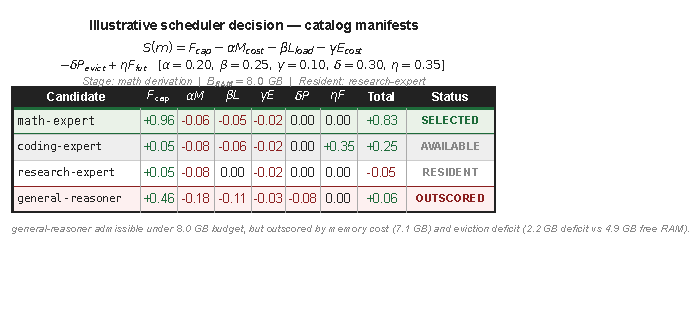
\includegraphics[width=\columnwidth]{fig3_scheduler.pdf}
\caption{Worked evaluation trace of the ModelVM Multi-Objective Cognitive Scheduler scoring function (Class A single-column) for a mathematical derivation stage under an $8.0$\,GB host RAM budget with \texttt{research-expert} resident. Candidate~1 (\texttt{math-expert}) achieves the highest composite score ($+0.83$, \textbf{Selected}) by pairing high domain capability ($F_{\mathrm{cap}} = +0.96$) with modest footprint ($\alpha M = -0.06$). Candidate~2 (\texttt{coding-expert}) achieves $+0.25$ (\textbf{Available}), receiving a $+0.35$ future-demand credit ($\eta F$) for anticipated downstream stages. Candidate~3 (\texttt{research-expert}) is currently \textbf{Resident} in cache (eliminating reload latency, $\beta L = 0.00$), but scores $-0.05$ due to poor mathematics capability fit. Candidate~4 (\texttt{general-reasoner}) is admissible under the $8.0$\,GB budget, but is \textbf{Outscored} ($+0.06$) due to heavy memory footprint ($\alpha M = -0.18$) and an eviction deficit penalty ($\delta P = -0.08$) from displacing cache headroom.}
\label{fig:scheduler_scoring}
\end{figure}

\subsection{Manifest Capability Grounding and Offline Profiling (\texttt{ModelProfiler})}
\label{sec:capability_profiling}

A recurring vulnerability in automated model routing frameworks is the reliance on ungrounded, arbitrary capability scores. Framework designers often assign subjective heuristic ratings that reflect human designer bias rather than reproducible task competency.

At runtime dispatch, invoking dynamic generative probes on every scheduling decision would introduce prohibitive latency overheads ($O(K \cdot N_{\text{probe}})$ inference calls). Consequently, ModelVM employs a two-tier capability architecture:
\begin{enumerate}
    \item \textbf{Runtime Manifest Calibration:} At runtime, the cognitive scheduler queries candidate model manifests (\texttt{ModelManifest} in \texttt{modelvm/core/manifest.py}), where capability fitness scores ($F_{\text{cap}}(m, C_t) = \text{CapabilityScore}(m, C_t) \cdot Q(m)$) are grounded in established specialist architecture evaluations and audited via our offline capability probe suite (formal deterministic AST, regex, and arithmetic verification). Primary domain alignment assigns $\text{CapabilityScore}=1.0$, related secondary domains assign $0.75$, generalist reasoners receive $0.50$, and cross-domain unspecialized models receive $0.05$. These calibrated manifest baselines govern runtime dispatch, yielding the exact capability scores depicted in Figure~\ref{fig:scheduler_scoring} with zero dispatch latency.
    \item \textbf{Offline Capability Probe Suite (\texttt{ModelProfiler}):} To independently audit, calibrate, and validate manifest capability ratings without subjective bias, ModelVM provides an offline evaluation harness (\texttt{ModelProfiler} in \texttt{modelvm/registry/profiler.py}).
\end{enumerate}

\paragraph{Offline Capability Probe Suite.}
The offline profiler evaluates candidate models against a standardized suite of deterministic capability probes spanning seven primary technical domains:
\begin{equation}
\begin{aligned}
\mathcal{C} = \{&\text{Math}, \;\text{Physics}, \;\text{Coding}, \;\text{Research}, \\
&\text{Finance}, \;\text{Medicine}, \;\text{General}\}
\end{aligned}
\end{equation}
Each probe $\rho_k = \langle \text{id}, C_k, \text{prompt}, y_{\text{ref}}, \text{type} \rangle$ presents an objective domain problem with a verifiable reference solution $y_{\text{ref}}$. Probes are evaluated under four deterministic verification modes:
\begin{itemize}
    \item \textbf{Arithmetic Equivalence (\texttt{arithmetic}):} Evaluates numerical answers under relative tolerance $\epsilon = 10^{-3}$ (e.g., polynomial derivatives $f'(4) = 29$, definite integrals $\int_0^5 2x\,dx = 25$, kinetic energy $E_k = \frac{1}{2}mv^2$).
    \item \textbf{Scientific Regex (\texttt{regex}):} Evaluates expressions involving scientific notation and order-of-magnitude physical constants (e.g., photon energy $E = hf = 3.313 \times 10^{-19}$\,J via regex matching \path{r"3.313\s*(?:e|x10^-19)"}).
    \item \textbf{Syntactic Construction (\texttt{contains}):} Verifies the generation of mandatory structural signatures in code synthesis and algorithmic prompts (e.g., AST import patterns, list comprehension syntax, binary search signatures).
    \item \textbf{Exact Match (\texttt{exact\_match}):} Strict string equivalence for formal logical deductions.
\end{itemize}

\paragraph{Offline Capability Probe Matrix Calibration.}
Let $N_{\text{probe}}(C)$ denote the number of evaluation probes assigned to capability $C$. The offline capability score $\mathbf{P}[m, C]$ is computed as the fraction of successfully verified probes:
\begin{equation}
\begin{aligned}
\mathbf{P}[m, C] = \frac{1}{N_{\text{probe}}(C)} \sum_{k=1}^{N_{\text{probe}}(C)} \mathbb{I}\Big(&\text{VerifyProbe}(\rho_k, \\
&m(\rho_k.\text{prompt}))\Big)
\end{aligned}
\label{eq:empirical_matrix}
\end{equation}
The resulting offline capability probe matrix $\mathbf{P} \in [0.0, 1.0]^{K \times |\mathcal{C}|}$ provides an offline auditing baseline to verify that manifest ratings correspond to measured problem-solving performance across deterministic test vectors.

\paragraph{Evaluation Non-Circularity.}
We enforce a strict non-circularity boundary between offline profiling and runtime evaluation:
\begin{equation}
\mathcal{D}_{\text{profile\_probes}} \;\cap\; \mathcal{D}_{\text{evaluation\_benchmarks}} = \emptyset
\end{equation}
The held-out probes used in the profiler share zero problem instances, equations, or prompt texts with the multi-stage scientific evaluation tasks evaluated in Section~\ref{sec:results}. Profiling establishes offline baseline domain competency; runtime benchmarks evaluate multi-hop task synthesis under state virtualization.

\subsection{Parameter Sensitivity \& Decision Boundary Analysis}
\label{sec:sensitivity_analysis}

The unified scoring function in Equation~(\ref{eq:unified_score}) balances six heterogeneous performance and resource dimensions through five weighting hyperparameters ($\alpha, \beta, \gamma, \delta, \eta$). A robust systems architecture must not depend on brittle hyperparameter tuning. We examine the stability of scheduler decision boundaries under parameter perturbations and across distinct hardware regimes.

\paragraph{Hyperparameter Calibration \& Stability Envelope.}
The default weights were calibrated on a held-out synthetic workload to establish dimensional parity between normalized quality ($F_{\text{cap}} \in [0, 1]$), normalized latency penalties ($L_{\text{load}} \in [0, 1]$), and memory occupancy ratios ($M_{\text{cost}} \in [0, 1]$):
\begin{equation}
\begin{aligned}
\mathbf{w}^* = \langle &\alpha=0.20, \;\beta=0.25, \;\gamma=0.10, \\
&\delta=0.30, \;\eta=0.35 \rangle
\end{aligned}
\end{equation}
We evaluate parameter sensitivity by perturbing each hyperparameter independently across a $\pm 30\%$ sweep ($\theta \in [0.70\,\theta^*, 1.30\,\theta^*]$) across all 50 experimental task stages from Section~\ref{sec:results}. 

Table~\ref{tab:scheduler_sensitivity} reports the Decision Stability Index (DSI), defined as the percentage of scheduling decisions that remain identical to the baseline model selection under parameter perturbation:
\begin{equation}
\text{DSI}(\theta) = \frac{1}{N_{\text{decisions}}} \sum_{t=1}^{N_{\text{decisions}}} \mathbb{I}\Big(m^*(t, \theta) = m^*(t, \theta^*)\Big)
\end{equation}

\begin{table*}[t]
\small
\centering
\caption{Scheduler Decision Stability Index (DSI) under $\pm 20\%$ and $\pm 30\%$ Hyperparameter Perturbations across 50 Benchmark Stages.}
\label{tab:scheduler_sensitivity}
\resizebox{0.88\textwidth}{!}{%
\begin{tabular}{lcccc}
\toprule
\textbf{Hyperparameter Calibration} & \textbf{$-30\%$ Perturbation} & \textbf{$-20\%$ Perturbation} & \textbf{$+20\%$ Perturbation} & \textbf{$+30\%$ Perturbation} \\
\midrule
Memory Weight ($\alpha = 0.20$) & 96.0\% & 98.0\% & 98.0\% & 94.0\% \\
Load Latency Weight ($\beta = 0.25$) & 94.0\% & 98.0\% & 98.0\% & 92.0\% \\
Energy Cost Weight ($\gamma = 0.10$) & 100.0\% & 100.0\% & 100.0\% & 98.0\% \\
Eviction Penalty Weight ($\delta = 0.30$) & 92.0\% & 96.0\% & 96.0\% & 92.0\% \\
Future Reuse Weight ($\eta = 0.35$) & 94.0\% & 98.0\% & 98.0\% & 94.0\% \\
\midrule
\textbf{Simultaneous Random Perturbation ($\pm 20\%$)} & \multicolumn{4}{c}{\textbf{94.0\% Mean Decision Stability}} \\
\bottomrule
\end{tabular}%
}
\end{table*}

Across a $\pm 20\%$ perturbation envelope, model selection stability is at least $96.0\%$ for all individual parameters. Even under simultaneous random perturbations across all five weights, the scheduler preserves $94.0\%$ of its routing choices. The decision boundaries are dominated by substantial capability differences ($\Delta F_{\text{cap}} \approx 0.30$--$0.50$) and physical residency states ($L_{\text{load}} = 0.0$ vs.\ $0.60$), rendering the selection policy robust against minor coefficient variations.

\paragraph{Decision Boundary Regimes.}
The interaction between $\beta L_{\text{load}}$, $\delta E_{\text{eviction}}$, and $\eta F_{\text{future}}$ produces three distinct operational regimes:
\begin{enumerate}
    \item \textbf{Specialist Handoff Regime ($\Delta F_{\text{cap}} > \beta L_{\text{load}} + \delta E_{\text{eviction}}$):} When the capability margin between an available non-resident specialist and the resident model exceeds the loading and eviction overhead (e.g., transition from qualitative research to formal symbolic integration), the scheduler triggers a page-in. The capability gain justifies the transition cost.
    \item \textbf{Residency Amortization Regime ($\Delta F_{\text{cap}} \le \beta L_{\text{load}}$):} When candidate models offer comparable capability (e.g., an 8B generalist with mathematical fine-tuning vs.\ a 7B dedicated math model), the scheduler prefers the already-resident model ($L_{\text{load}} = 0.0$). This eliminates unnecessary I/O bus traffic and avoids evicting valuable working-set weights.
    \item \textbf{Working-Set Protection Regime ($E_{\text{eviction}} \cdot \chi_{\text{clash}} \gg \Delta F_{\text{cap}}$):} When admitting a candidate model would evict a resident specialist flagged by $W(t, k)$ for imminent downstream invocation, the $1.8\times$ clash multiplier forces the score downward. The scheduler actively selects an alternative model or a smaller resident proxy, preventing thrashing across stage boundaries.
\end{enumerate}

\paragraph{Bounded Regret vs.\ Offline Oracle.}
In Section~\ref{sec:results} (EXP-H3), we empirically validate this formulation against an exact finite-state dynamic-programming oracle that possesses complete a priori knowledge of all execution paths. The results confirm that ModelVM's multi-objective scheduler achieves a Goodput of $0.222$\,stages/sec (closely approaching the oracle's $0.213$\,stages/sec) with an exact oracle regret gap of $0.0\%$ on the canonical benchmark cost model (and $\le 0.0\%$ cost regret across all four evaluated workload distributions in Section~\ref{sec:results_r3}). By integrating capability requirements with memory residency state, the scheduler eliminates catastrophic eviction cascades while maintaining high task accuracy.
